\chapter{Acids and Bases: Ka and pKa}\label{ch:g12:ka-and-pka}

Many ants defend themselves with methanoic acid, and on the skin it
burns. Methanoic acid is a small
\omterm{def:g11:functional-groups:carboxylic-acid}{carboxylic acid}. Hydrochloric acid at the same concentration would burn
far more. Both are acids; both give a solution of \omterm{def:g9:acids-bases-ph:ph}{pH} below 7; yet they are
not acidic in the same way. To describe an acid fully, two numbers are
needed: how much of it there is, its concentration, and how readily it
gives away its hydrogen \omterm{def:g9:ions:ion}{ion}, its \omterm{def:g12:ka-and-pka:ka}{acidity constant}.

\begin{recall}
Acidic, basic and \omterm{def:g9:acids-bases-ph:acidic}{neutral solutions}; the \omterm{def:g9:acids-bases-ph:ph}{pH} scale, from 0 to 14, lower
when there are more hydrogen \omterm{def:g9:ions:ion}{ions} (\cref{ch:g9:acids-bases-ph}). The
\omterm{def:g12:equilibrium:quotient}{reaction quotient} $Q$ and the \omterm{def:g12:equilibrium:constant}{equilibrium constant} $K$
(\cref{ch:g12:equilibrium}). A \omterm{def:g12:curly-arrows:curly-arrow}{curly arrow} shows a pair of \omterm{def:g9:inside-the-atom:nucleus}{electrons}
moving (\cref{ch:g12:curly-arrows}).
\end{recall}

\begin{omfigure}
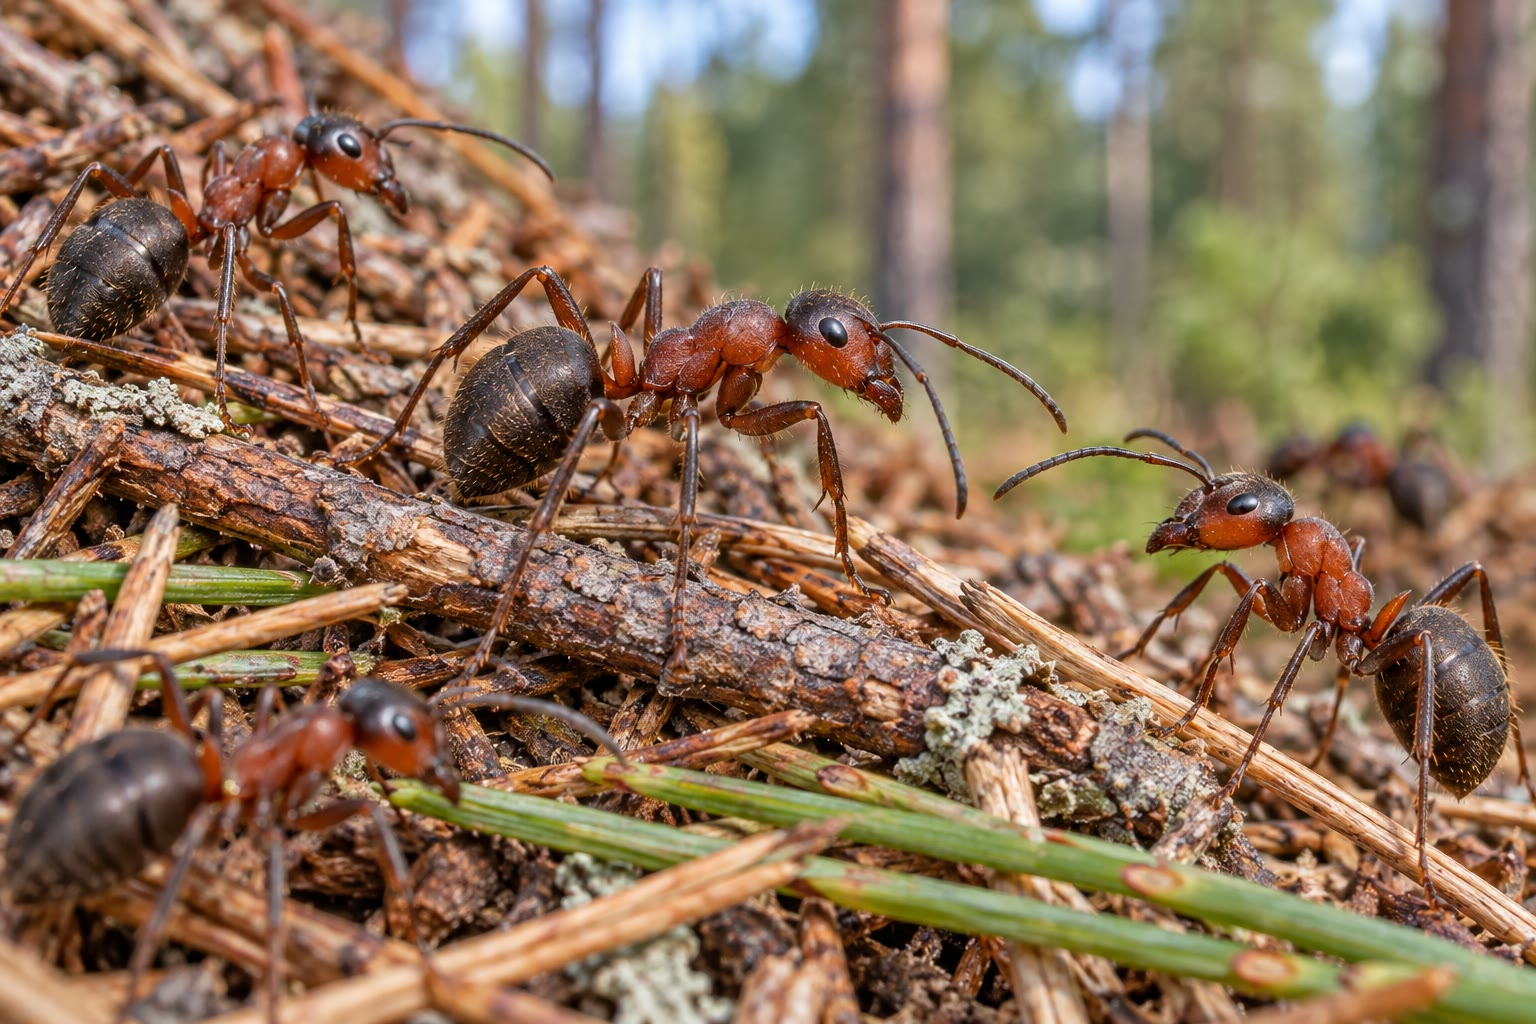
\includegraphics[width=0.45\linewidth]{images/book1/ai/g12-red-ants.jpg}

{\small Wood ants: like many ants, they defend themselves with methanoic acid.}
\end{omfigure}

\section{Brønsted acids and bases}

\begin{definition}[Brønsted acid and base, acid--base couple]\label{def:g12:ka-and-pka:bronsted}
A \emph{Brønsted acid}\index{Brønsted acid} is a species able to give a
hydrogen \omterm{def:g9:ions:ion}{ion} \ce{H+}; a \emph{Brønsted base}\index{Brønsted base} is a
species able to take one. An acid HA and the base \ce{A-} it becomes by
losing \ce{H+} form an \emph{acid--base couple}\index{acid--base couple},
written \ce{HA}/\ce{A-}: $\ce{HA} \rightleftharpoons \ce{A-} + \ce{H+}$.
\end{definition}

\begin{definition}[Oxonium ion, ampholyte]\label{def:g12:ka-and-pka:oxonium}
In water a hydrogen \omterm{def:g9:ions:ion}{ion} never stays alone: it is taken by a water
\omterm{def:g7:atoms-and-molecules:molecule}{molecule}, giving the \emph{oxonium ion}\index{oxonium ion} \ce{H3O+}. A
species that is the acid of one couple and the base of another is an
\emph{ampholyte}\index{ampholyte}; water is one, acid of the couple
\ce{H2O}/\ce{OH-} and base of the couple \ce{H3O+}/\ce{H2O}.
\end{definition}

\begin{example}[An acid in water]\label{ex:g12:ka-and-pka:acid-water}
When ethanoic acid \omterm{def:g2:mixing-and-dissolving:dissolve}{dissolves}, a \omterm{def:g10:lewis-and-shape:lone-pair}{lone pair} of a water \omterm{def:g7:atoms-and-molecules:molecule}{molecule} takes the
hydrogen of its \ce{O-H}, and the \ce{O-H} pair stays on the acid's oxygen:
\[
  \ce{CH3COOH + H2O <=> CH3COO- + H3O+} .
\]
Two couples exchange a hydrogen \omterm{def:g9:ions:ion}{ion}: \ce{CH3COOH}/\ce{CH3COO-} gives it,
\ce{H3O+}/\ce{H2O} takes it. From now on, the hydrogen \omterm{def:g9:ions:ion}{ions} of earlier
chapters are written \ce{H3O+} whenever water is the \omterm{def:g6:solutions-and-solubility:solute}{solvent}.
\end{example}

\begin{omfigure}
\setchemfig{atom sep=2em}
\chemfig{H_3C-C(=[2]O)-O-[@{oh}]@{h}H}\qquad
\chemfig{@{ow}\charge{90=\:,270=\:}{O}(-[:150]H)-[:210]H}
\qquad$\longrightarrow$\qquad
\chemfig{H_3C-C(=[2]O)-\charge{90=\:,0=\:,270=\:}{O}^{-}}\quad$+$\quad\ce{H3O+}
\chemmove{
  \draw[->, thick, omProp, shorten <=4pt, shorten >=3pt]
    ($(ow)+(0,0.25)$) .. controls +(110:9mm) and +(60:9mm) .. (h);
  \draw[->, thick, omDef, shorten <=2pt, shorten >=4pt]
    (oh) .. controls +(-90:7mm) and +(-60:6mm) .. ($(oh)+(-0.3,-0.2)$);}

{\small A hydrogen \omterm{def:g9:ions:ion}{ion} passes from the acid to water: a \omterm{def:g10:lewis-and-shape:lone-pair}{lone pair} of
water forms the new \ce{O-H} bond (orange), and the old \ce{O-H} pair
stays on the oxygen of the ethanoate \omterm{def:g9:ions:ion}{ion} (blue).}
\end{omfigure}

\begin{history}[From Arrhenius to Brønsted, 1887--1923]
In 1887 Svante Arrhenius proposed that acids give hydrogen \omterm{def:g9:ions:ion}{ions} in water
and bases hydroxide \omterm{def:g9:ions:ion}{ions}. In 1923 Johannes Brønsted, and independently
Thomas Lowry, broadened the idea: an acid is any species that gives a
hydrogen \omterm{def:g9:ions:ion}{ion}, a base any species that takes one, in water or not. The
ammonia \omterm{def:g7:atoms-and-molecules:molecule}{molecule}, which contains no hydroxide, became a base like any
other.
\end{history}

\begin{omfigure}
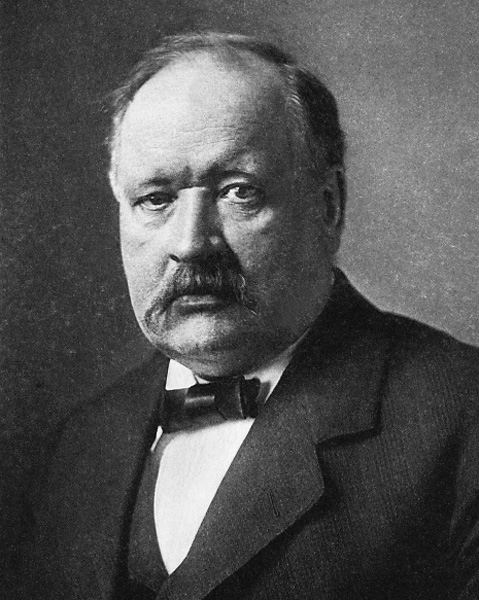
\includegraphics[width=0.22\linewidth]{images/book1/arrhenius.jpg}

{\small Svante Arrhenius (1859--1927).}
\end{omfigure}

\section{The pH, quantitatively}

\begin{definition}[The pH, precisely]\label{def:g12:ka-and-pka:ph-log}
In a dilute \omterm{def:g6:solutions-and-solubility:solute}{aqueous solution}, the \omterm{def:g9:acids-bases-ph:ph}{pH} is defined by
\[
  \mathrm{pH} = -\log\frac{[\ce{H3O+}]}{c^\circ},
  \qquad\text{that is}\qquad
  [\ce{H3O+}] = c^\circ \times 10^{-\mathrm{pH}} ,
\]
where $\log$ is the decimal logarithm.
\end{definition}

\begin{proposition}[Tenfold dilution, one unit]\label{prop:g12:ka-and-pka:dilution}
If $[\ce{H3O+}]$ is divided by 10, the \omterm{def:g9:acids-bases-ph:ph}{pH} increases by 1; if it is
multiplied by 10, the \omterm{def:g9:acids-bases-ph:ph}{pH} decreases by 1.
\end{proposition}

\begin{proof}
$-\log\big([\ce{H3O+}]/10c^\circ\big) = -\log\big([\ce{H3O+}]/c^\circ\big)
+ \log 10 = \mathrm{pH} + 1$.
\end{proof}

\begin{definition}[Strong and weak acids and bases]\label{def:g12:ka-and-pka:strong-acid}
A \emph{strong acid}\index{strong acid} reacts totally with water: none
of the acid remains as such in the solution. A \emph{weak
acid}\index{weak acid} reacts partially: its reaction with water reaches
an equilibrium. Likewise a \emph{strong base}\index{strong base} reacts
totally with water, a \emph{weak base}\index{weak base} partially.
\end{definition}

\begin{proposition}[pH of a strong acid]\label{prop:g12:ka-and-pka:strong}
A solution of a \omterm{def:g12:ka-and-pka:strong-acid}{strong acid} of concentration $c$ (not too dilute) has
$[\ce{H3O+}] = c$ and $\mathrm{pH} = -\log(c/c^\circ)$.
\end{proposition}

\begin{proof}
The reaction \ce{HA + H2O -> A- + H3O+} is total: each \omterm{def:g7:atoms-and-molecules:molecule}{molecule} of acid
gives one \omterm{def:g12:ka-and-pka:oxonium}{oxonium ion}. The \omterm{def:g9:ions:ion}{ions} coming from water itself are negligible
as long as $c$ is much larger than \qty{e-7}{mol/L}.
\end{proof}

\begin{example}[Hydrochloric acid]\label{ex:g12:ka-and-pka:hcl}
Hydrochloric acid at \qty{0.010}{mol/L}: $[\ce{H3O+}] = \qty{0.010}{mol/L}$
and $\mathrm{pH} = -\log 0.010 = 2.0$. Diluted ten times, \omterm{def:g9:acids-bases-ph:ph}{pH} 3.0.
\end{example}

\section{Water and the ionic product}


\begin{definition}[Ionic product of water]\label{def:g12:ka-and-pka:ionic-product}
Water reacts very slightly with itself, \ce{2H2O <=> H3O+ + OH-}. The
\omterm{def:g12:equilibrium:constant}{equilibrium constant} of this reaction is the \emph{ionic product of
water}\index{ionic product of water}:
\[
  K_e = \frac{[\ce{H3O+}]\,[\ce{OH-}]}{(c^\circ)^2},
  \qquad pK_e = -\log K_e .
\]
\end{definition}

\begin{proposition}[Neutral water and strong bases]\label{prop:g12:ka-and-pka:ke}
% ledger: ke:25C
At \qty{25}{\celsius}, $K_e = \num{1.0e-14}$ and $pK_e = 14.0$. In pure
water $[\ce{H3O+}] = [\ce{OH-}] = \qty{1.0e-7}{mol/L}$: \omterm{def:g9:acids-bases-ph:ph}{pH} 7.0. A \omterm{def:g12:ka-and-pka:strong-acid}{strong
base} of concentration $c$ gives $[\ce{OH-}] = c$, so
$[\ce{H3O+}] = K_e (c^\circ)^2 / c$ and $\mathrm{pH} = 14.0 + \log(c/c^\circ)$.
\end{proposition}

\begin{proof}
In pure water the two \omterm{def:g9:ions:ion}{ions} come in pairs, so they are equal, and their
product is $\num{1.0e-14}$: each is \qty{1.0e-7}{mol/L}. For the base,
$K_e$ still holds in the solution:
$-\log([\ce{H3O+}]/c^\circ) = -\log K_e + \log(c/c^\circ)$.
\end{proof}

\begin{example}[Sodium hydroxide]\label{ex:g12:ka-and-pka:naoh}
Sodium hydroxide at \qty{0.010}{mol/L}: $[\ce{OH-}] = 0.010$, so
$[\ce{H3O+}] = \num{1.0e-14}/0.010 = \qty{1.0e-12}{mol/L}$ and \omterm{def:g9:acids-bases-ph:ph}{pH} 12.0.
\end{example}

\section{The acidity constant}

\begin{definition}[Acidity constant, $pK_a$]\label{def:g12:ka-and-pka:ka}
The \emph{acidity constant}\index{acidity constant} $K_a$ of a couple
\ce{HA}/\ce{A-} is the \omterm{def:g12:equilibrium:constant}{equilibrium constant} of the reaction of the acid
with water, \ce{HA + H2O <=> A- + H3O+}:
\[
  K_a = \frac{[\ce{A-}]\,[\ce{H3O+}]}{[\ce{HA}]\,c^\circ} .
\]
The \emph{pKa}\index{pKa} of the couple is
$pK_a = -\log K_a$.
\end{definition}

\begin{proposition}[The smaller the $pK_a$, the stronger the acid]\label{prop:g12:ka-and-pka:compare}
Of two \omterm{def:g12:ka-and-pka:strong-acid}{weak acids} at the same concentration, the one with the larger
$K_a$, that is the smaller $pK_a$, reacts more with water and gives the
lower \omterm{def:g9:acids-bases-ph:ph}{pH}; its conjugate base is the weaker.
\end{proposition}

\begin{proof}
A larger $K_a$ means more \ce{A-} and \ce{H3O+} at equilibrium for the
same \ce{HA}. The base \ce{A-} of a couple that gives up its hydrogen \omterm{def:g9:ions:ion}{ion}
easily takes it back reluctantly.
\end{proof}

\begin{omfigure}
\begin{tikzpicture}[font=\small, y=0.55cm]
  % ledger: pka:methanoic, pka:ethanoic, pka:benzoic, pka:ascorbic1, ka:HF, ka:H2CO3, ka:HCO3, kb:NH3, ke:25C
  \draw[->, thick] (0,0) -- (0,14.8) node[above] {$pK_a$};
  \foreach \k in {0,2,4,6,8,10,12,14} \draw (-0.1,\k) -- (0.1,\k) node[right, font=\scriptsize] {\k};
  \node[font=\footnotesize\bfseries, anchor=south] at (-3.0,14.3) {acid};
  \node[font=\footnotesize\bfseries, anchor=south] at (3.0,14.3) {base};
  \foreach \p/\yl/\acid/\base in {3.19/2.9/{\ce{HF}}/{\ce{F-}},
      3.74/3.6/{\ce{HCOOH}}/{\ce{HCOO-}}, 4.04/4.3/{ascorbic acid}/{ascorbate},
      4.20/5.0/{\ce{C6H5COOH}}/{\ce{C6H5COO-}}, 4.76/5.7/{\ce{CH3COOH}}/{\ce{CH3COO-}},
      6.37/6.9/{\ce{CO2,H2O}}/{\ce{HCO3-}}, 9.26/9.26/{\ce{NH4+}}/{\ce{NH3}},
      10.33/10.4/{\ce{HCO3-}}/{\ce{CO3^{2-}}}} {
    \draw[omDef] (-0.25,\p) -- (0.25,\p);
    \draw[black!40] (-0.25,\p) -- (-1.1,\yl);
    \draw[black!40] (0.25,\p) -- (1.1,\yl);
    \node[anchor=east, font=\scriptsize] at (-1.15,\yl) {\acid};
    \node[anchor=west, font=\scriptsize] at (1.15,\yl) {\base};
  }
  \draw[->, omThm, thick] (-4.6,13) -- (-4.6,1);
  \node[omThm, rotate=90, font=\footnotesize] at (-4.95,7) {stronger acids};
  \draw[->, omMeth, thick] (4.6,1) -- (4.6,13);
  \node[omMeth, rotate=90, font=\footnotesize] at (4.95,7) {stronger bases};
\end{tikzpicture}

{\small Some couples placed by their $pK_a$ at \qty{25}{\celsius}, acids
on the left, their bases on the right. The lower a couple on the scale,
the stronger its acid; the higher, the stronger its base.}
\end{omfigure}


\begin{method}[pH of a weak acid]\label{met:g12:ka-and-pka:weak}
For a \omterm{def:g12:ka-and-pka:strong-acid}{weak acid} of concentration $c$ and constant $K_a$:
\begin{enumerate}
  \item Write the \omterm{def:g10:reaction-progress-table:extent}{progress table} of \ce{HA + H2O <=> A- + H3O+} per litre,
        with $x = [\ce{H3O+}]$: $[\ce{HA}] = c - x$, $[\ce{A-}] = x$
        (water's own \omterm{def:g9:ions:ion}{ions} neglected).
  \item Solve $\dfrac{x^2}{(c - x)\,c^\circ} = K_a$, the quadratic
        $x^2 + K_a c^\circ x - K_a c^\circ c = 0$, keeping the positive
        root.
  \item $\mathrm{pH} = -\log(x/c^\circ)$; check that $x$ is much larger
        than \qty{e-7}{mol/L}.
\end{enumerate}
\end{method}

\begin{example}[Ethanoic acid at \texorpdfstring{\qty{0.010}{mol/L}}{0.010 mol/L}]\label{ex:g12:ka-and-pka:acetic}
% ledger: pka:ethanoic
$pK_a = 4.76$, so $K_a = 10^{-4.76} = \num{1.74e-5}$. Then
$x^2 + \num{1.74e-5}\,x - \num{1.74e-7} = 0$ gives
$x = \qty{4.1e-4}{mol/L}$ and \omterm{def:g9:acids-bases-ph:ph}{pH} 3.39. Only $\num{4.1e-4}/0.010 =
\qty{4.1}{\percent}$ of the acid has reacted with water; hydrochloric
acid at the same concentration, \omterm{def:g9:acids-bases-ph:ph}{pH} 2.0, has reacted entirely.
\end{example}

\begin{omfigure}
\begin{tikzpicture}[font=\small]
  \fill[omThm!45] (0,1.3) rectangle (8,2.0);
  \node[anchor=east] at (-0.1,1.65) {\ce{HCl}, \qty{0.010}{mol/L}};
  \node[white, font=\small\bfseries] at (4,1.65) {\ce{H3O+} + \ce{Cl-}: \qty{100}{\percent}};
  \fill[omDef!35] (0,0) rectangle (7.67,0.7);
  \fill[omThm!45] (7.67,0) rectangle (8,0.7);
  \node[anchor=east] at (-0.1,0.35) {\ce{CH3COOH}, \qty{0.010}{mol/L}};
  \node at (3.8,0.35) {\ce{CH3COOH} left as such: \qty{95.9}{\percent}};
  \draw[<-, omThm] (7.85,0.75) -- (8.4,1.1) node[right, font=\footnotesize] {\qty{4.1}{\percent} ionised};
\end{tikzpicture}

{\small What becomes of a strong and a \omterm{def:g12:ka-and-pka:strong-acid}{weak acid} at the same
concentration: the \omterm{def:g12:ka-and-pka:strong-acid}{strong acid} is entirely turned into \omterm{def:g9:ions:ion}{ions}, the \omterm{def:g12:ka-and-pka:strong-acid}{weak
acid} hardly at all. Hence the \omterm{def:g9:acids-bases-ph:ph}{pH} difference, 2.0 against 3.4.}
\end{omfigure}

\begin{safety}{\ghs[0.75cm]{GHS02}\ghs[0.75cm]{GHS05}\ghs[0.75cm]{GHS06}\ghs[0.75cm]{GHS07}}
% ledger: ghs:formic-acid
Concentrated methanoic acid is flammable, causes severe burns of the skin
and the eyes, and its vapour is toxic. It is handled only by the teacher,
under a fume hood; the dilute solutions of the exercises still need
goggles.
\end{safety}

\section{Exercises}

\begin{exercise}[$\star$]\label{exo:g12:ka-and-pka:1}
Give the conjugate base of: \ce{HCOOH}, \ce{NH4+}, \ce{H2O}, \ce{HCO3-};
and the conjugate acid of: \ce{NH3}, \ce{OH-}, \ce{H2O}, \ce{HCO3-}.
Which species are \omterm{def:g12:ka-and-pka:oxonium}{ampholytes}?
\end{exercise}

\begin{exercise}[$\star$]\label{exo:g12:ka-and-pka:2}
Compute the \omterm{def:g9:acids-bases-ph:ph}{pH} of hydrochloric acid at \qty{0.10}{mol/L},
\qty{0.0010}{mol/L} and \qty{5.0e-3}{mol/L}.
\end{exercise}

\begin{exercise}[$\star$]\label{exo:g12:ka-and-pka:3}
A solution has \omterm{def:g9:acids-bases-ph:ph}{pH} 4.5. Compute $[\ce{H3O+}]$. A solution has \omterm{def:g9:acids-bases-ph:ph}{pH} 11.2:
compute $[\ce{H3O+}]$ and $[\ce{OH-}]$ at \qty{25}{\celsius}.
\end{exercise}

\begin{exercise}[$\star$]\label{exo:g12:ka-and-pka:4}
Write the reaction with water and the expression of $K_a$ for methanoic
acid and for the ammonium \omterm{def:g9:ions:ion}{ion}.
\end{exercise}

\begin{exercise}[$\star$]\label{exo:g12:ka-and-pka:5}
Which is the stronger acid: methanoic acid ($pK_a = 3.74$) or ethanoic
acid ($pK_a = 4.76$)? Which is the stronger base: \ce{HCOO-} or
\ce{CH3COO-}?
\end{exercise}

\begin{exercise}[$\star\star$]\label{exo:g12:ka-and-pka:6}
A solution of a \omterm{def:g12:ka-and-pka:strong-acid}{weak acid} HA at \qty{0.050}{mol/L} has \omterm{def:g9:acids-bases-ph:ph}{pH} 3.0. Compute
$[\ce{A-}]$, $[\ce{HA}]$, then $K_a$ and $pK_a$.
\end{exercise}

\begin{exercise}[$\star\star$]\label{exo:g12:ka-and-pka:7}
Compute the \omterm{def:g9:acids-bases-ph:ph}{pH} of benzoic acid at \qty{0.020}{mol/L} ($pK_a = 4.20$).
\end{exercise}

\begin{exercise}[$\star\star$]\label{exo:g12:ka-and-pka:8}
Compute the \omterm{def:g9:acids-bases-ph:ph}{pH} of a sodium hydroxide solution at \qty{2.0e-3}{mol/L}.
\end{exercise}

\begin{exercise}[$\star\star$]\label{exo:g12:ka-and-pka:9}
Using the $pK_a$ scale, list the acids of the couples shown from the
strongest to the weakest. Where would a \omterm{def:g12:ka-and-pka:strong-acid}{strong acid} such as \ce{HCl}
lie?
\end{exercise}

\begin{exercise}[$\star\star$]\label{exo:g12:ka-and-pka:10}
Carbon dioxide dissolved in water makes it slightly acidic (couple
\ce{CO2,H2O}/\ce{HCO3-}, $pK_a = 6.37$). A sample of rain water in contact with the
\omterm{def:g4:air-a-mixture-of-gases:air}{air} is found to have \omterm{def:g9:acids-bases-ph:ph}{pH} 5.6. Compute $[\ce{H3O+}]$, and compare with pure water.
\end{exercise}

\begin{exercise}[$\star\star$]\label{exo:g12:ka-and-pka:11}
Show that for the couple \ce{NH4+}/\ce{NH3}, $pK_a = pK_e - pK_b$, where
$K_b = \num{1.8e-5}$ is the constant of \ce{NH3 + H2O <=> NH4+ + OH-}.
Compute the $pK_a$.
\end{exercise}

\begin{exercise}[$\star\star\star$]\label{exo:g12:ka-and-pka:12}
Ethanoic acid at \qty{0.010}{mol/L} has \omterm{def:g9:acids-bases-ph:ph}{pH} 3.39. Compute the \omterm{def:g9:acids-bases-ph:ph}{pH} after a
tenfold \omterm{def:g10:concentration-and-dilution:dilution}{dilution}. Does it rise by one unit, as for a \omterm{def:g12:ka-and-pka:strong-acid}{strong acid}?
Explain.
\end{exercise}

\begin{exercise}[$\star\star\star$]\label{exo:g12:ka-and-pka:13}
The hydrogencarbonate \omterm{def:g9:ions:ion}{ion} is an \omterm{def:g12:ka-and-pka:oxonium}{ampholyte}. Write its two reactions with
water and their constants, using the $pK_a$ scale. Which is larger?
What does that suggest for the \omterm{def:g9:acids-bases-ph:ph}{pH} of a sodium hydrogencarbonate
solution?
\end{exercise}

\begin{exercise}[$\star\star\star$]\label{exo:g12:ka-and-pka:14}
Hydrochloric acid at \qty{1.0e-3}{mol/L} is diluted a thousand times,
then a thousand times again. A careless rule gives \omterm{def:g9:acids-bases-ph:ph}{pH} 6, then \omterm{def:g9:acids-bases-ph:ph}{pH} 9. Why is
\omterm{def:g9:acids-bases-ph:ph}{pH} 9 impossible for a diluted acid? What \omterm{def:g9:acids-bases-ph:ph}{pH} does the very dilute solution
approach?
\end{exercise}

\begin{exercise}[$\star\star\star$]\label{exo:g12:ka-and-pka:15}
Ascorbic acid (vitamin C, $pK_a = 4.04$, $M = \qty{176.0}{g/mol}$): a
tablet of \qty{500}{mg} is dissolved in \qty{200}{mL} of water. Compute
the \omterm{def:g9:acids-bases-ph:ph}{pH} (consider only the first acidity).
\end{exercise}

\section{Problem: The Ant's Venom}


\begin{problem}[{Weekend problem --- what pH does the methanoic acid of an
ant's venom give at 0.010 mol/L, and how does baking soda soothe its burn?}]
\label{pb:g12:ka-and-pka:1}
% ledger: src:formic-ants, pka:methanoic, ka:H2CO3, ke:25C, aw:C, aw:H, aw:O
Methanoic acid, \ce{HCOOH}, is found in the venom of ants. Its $pK_a$ at
\qty{25}{\celsius} is 3.74. We study a solution at \qty{0.010}{mol/L} and
compare it with hydrochloric acid.

\medskip
\noindent\textbf{Part I --- The acid.}
\begin{enumerate}
  \item Draw the \omterm{def:g10:lewis-and-shape:lewis-structure}{Lewis structure} of methanoic acid and circle the
        hydrogen it gives.
  \item Write its couple and its reaction with water.
  \item Write $K_a$ and compute its value.
  \item Place the couple on the $pK_a$ scale: is methanoic acid stronger
        or weaker than ethanoic acid?
  \item Compute the mass of methanoic acid in \qty{1.0}{L} of the
        solution.
\end{enumerate}

\medskip
\noindent\textbf{Part II --- The \omterm{def:g9:acids-bases-ph:ph}{pH}.}
\begin{enumerate}[resume]
  \item Fill the \omterm{def:g10:reaction-progress-table:extent}{progress table} per litre, with $x = [\ce{H3O+}]$.
  \item Write the equation $Q_{eq} = K_a$.
  \item Solve it.
  \item Compute the \omterm{def:g9:acids-bases-ph:ph}{pH}.
  \item What fraction of the acid has reacted with water?
  \item Check that the \omterm{def:g9:ions:ion}{ions} coming from water can be neglected.
\end{enumerate}

\medskip
\noindent\textbf{Part III --- Comparison.}
\begin{enumerate}[resume]
  \item What is the \omterm{def:g9:acids-bases-ph:ph}{pH} of hydrochloric acid at \qty{0.010}{mol/L}?
  \item How many times more \omterm{def:g12:ka-and-pka:oxonium}{oxonium ions} does it contain than the
        methanoic acid solution?
  \item Explain the difference, using the words strong and weak.
\end{enumerate}

\medskip
\noindent\textbf{Part IV --- Baking soda.}
\begin{enumerate}[resume]
  \item Baking soda is sodium hydrogencarbonate. Write the reaction
        between methanoic acid and the hydrogencarbonate \omterm{def:g9:ions:ion}{ion} (it gives
        methanoate and \ce{CO2,H2O}).
  \item Show that its constant is $K = K_a(\ce{HCOOH}) / K_a(\ce{CO2,H2O})$,
        and compute it.
  \item Is the reaction favourable? What gas is seen?
  \item Why is a base much weaker than hydroxide, such as hydrogencarbonate,
        preferred on the skin?
  \item State the final answer: what is the \omterm{def:g9:acids-bases-ph:ph}{pH} of a \qty{0.010}{mol/L}
        methanoic acid solution?
\end{enumerate}
\end{problem}
